\documentclass[letterpaper,10pt]{article}
\usepackage{graphicx}
\usepackage{listings}

\title{Angular contact with TensorFlow}
\author{Rocco Malisi}

\begin{document}
	\maketitle
	\newpage
	
	\begin{abstract}
		Abstract text here alsdjfsdalsdjlfksdjlk
	\end{abstract}
	\newpage
	
	\tableofcontents
	\newpage
	
	\section{Introduction}
	Topics that should be covered here: EDA, tensorflow, python tools: (jupyter, matplotlib, numpy, pandas, scikitlearn), ml topics (activation function, evaluation metrics, optimizers,...)
	\section{Methods}
	\section{Results}
	\subsection{Performing an EDA on dataset \#1}
	To get a better understanding of dataset \#1, an EDA is performed. The objective is to identify patterns and relationships in the data. The insights gained by this analysis will be used in building and improving the model.
	\newline The dataset consists of three columns and 1365 rows. The columns are 'Fr' (radial force in N[Newton]), 'n' (rotational speed in rpm[revolutions per minute]) and 'Lifetime' (lifetime in h[hours]). The dataset does not contain any empty or null values and therefore does not require cleaning.
	\newline Figure 1 shows a plot of column Fr. The value of Fr starts at 200 and is increased by 100 every 35 rows throughout the whole dataset. The final and highest value of Fr is 4000. 
	\newline The column Lifetime is shown in figure 3. The highest value at the first row is 88445568 but it drops rapidly throughout the dataset to just 116 in the last row. Every 35 rows the value has a local peak but then quickly drops again. Figure 2 is a plot of rows 1000 and up which shows that this trend continues all the way throughout the dataset even though it can't be seen when plotting all rows. 
	\newline The column n is shown in figure 4. The value of n follows a pattern which repeats every 35 rows for 39 times. From the starting value of 100, n is  increased linearly to its peak value of 3500, after which it drops back to 100 and the next iteration begins. 
	\newline These findings already give insights about potential relationships of the variables. The peaks in the value of lifetime appear when n is at its lowest at 100. When n increases, the peak in lifetime drops sharply. This could be due to the increased load on the bearing system as n increases. As Fr steadily increases throughout the dataset, the peaks of lifetime become smaller even though n follow the same pattern. Therefore Fr must also have a negative correlation with lifetime.
	\newline Figure 5 shows the correlation matrix of the dataset. Both Fr and n show a weak negative correlation with lifetime of -0.21 and -0.12, respectively. 
	
	
	
	
	
	
	
	
	
	
	
	
	
	
	
	
	
	
	
	\subsection{Building the first model on dataset \#1}
	This chapter is about building the first model on dataset \#1. It will predict the lifetime of the bearing system using Fr and n as input features. The EDA already showed that the dataset does not require cleaning or further preprocessing.
	\newline This first model will be a simple neural network. To improve the models accuracy, the number of hidden layers and the number of neurons per hidden layer were tested in different combinations. The best accuracy in predicting the lifetime was achieved with the following configuration: 
	\begin{itemize}
		\item Input layer with 2 neurons for features Fr and n
		\item First hidden layer with 512 neurons and activation function ReLU
		\item Second hidden layer with 512 neurons and activation function ReLU
		\item Output layer with 1 neuron predicting the value of lifetime
	\end{itemize} 
	\ \\The code used to build the model architecture:
	\begin{lstlisting}
		model = tf.keras.Sequential([
		layers.Dense(512, activation='relu', input_shape=[2]), 
		layers.Dense(512, activation='relu'),  
		layers.Dense(1)
		])
	\end{lstlisting}
	The next step is model compilation which includes defining the loss function, optimizer and metrics. The model uses mean absolute percentage error as its loss function, the Adam algorithm as its optimizer and mean average percentage error as evaluation metric. 
	\\ \\ The code used to compile the model:
	\begin{lstlisting}
		model.compile(loss='mean_absolute_percentage_error',
		optimizer=tf.keras.optimizers.Adam(),
		metrics=[tf.keras.metrics.MeanAbsolutePercentageError()],
		run_eagerly=True)
	\end{lstlisting}
	In the final step, the dataset will be prepared and used for training and evaluating the model. First the dataset is split up into training and test data using the scikit-learn train\textunderscore test\textunderscore split function with a train\textunderscore size of 0.8 and a test\textunderscore size of 0.2. The split data is then used to train and evaluate the model. The mean absolute error metric is used to evaluate the model.
	\\ \\ The code to train and evaluate the model:
	\begin{lstlisting}
		X_train, X_test, y_train, y_test = 
		train_test_split(dataset[['Fr', 'n']], dataset['Lifetime'], 
		shuffle=True, 
		train_size=0.8, 
		test_size=0.2)
		
		model.fit(X_train, y_train, epochs=10, verbose=0)
		
		test_loss = model.evaluate(X_test, y_test)
	\end{lstlisting} 
	The evaluation error of this model is 68\% using the mean average percentage error metric. This means that the models predicted value of lifetime is off by 68\% on average.
	
	
	
	
	
	
	
	
	
	
	
	
	
	
	
	
	
	
	
	
	
	
	
	
	
	
	
	
	
	
	
	
	
	\begin{figure}
		\caption{Plot of Fr}
		\centering
		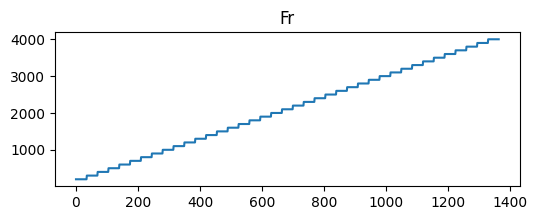
\includegraphics[scale=0.65]{assets/dataset1_column_Fr_plot.png}
	\end{figure}
	\begin{figure}
		\caption{Plot of Lifetime}
		\centering
		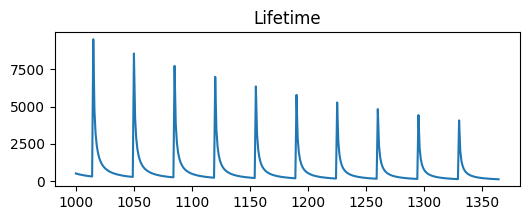
\includegraphics[scale=0.65]{assets/dataset1_column_Lifetime_plot2.png}
	\end{figure}
	\begin{figure}
		\caption{Plot of Lifetime}
		\centering
		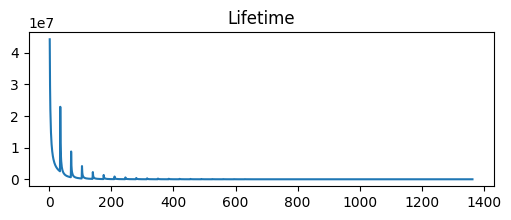
\includegraphics[scale=0.65]{assets/dataset1_column_Lifetime_plot1.png}
	\end{figure}
	\begin{figure}
		\caption{Plot of n}
		\centering
		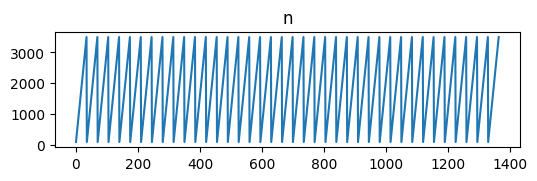
\includegraphics[scale=0.65]{assets/dataset1_column_n_plot.png}
	\end{figure}
	\begin{figure}
		\caption{Correlation matrix of dataset \#1}
		\centering
		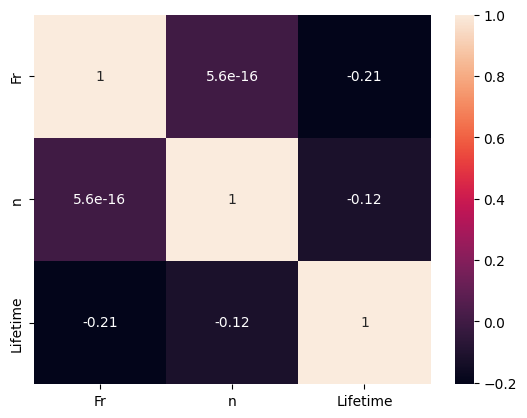
\includegraphics[scale=0.5]{assets/dataset1_correlation_matrix.png}
	\end{figure}

	\newpage
	\bibliographystyle{plain} 
	\bibliography{bibliography}
	
\end{document}